\documentclass[conference]{IEEEtran}
\IEEEoverridecommandlockouts
\usepackage{cite}
\usepackage{amsmath,amssymb,amsfonts}
\usepackage{algorithmic}
\usepackage{graphicx}
\usepackage{textcomp}
\usepackage{xcolor}
\usepackage{booktabs}
\usepackage{array}
\graphicspath{{./}{results/figures/}}
\def\BibTeX{{\rm B\kern-.05em{\sc i\kern-.025em b}\kern-.08em
    T\kern-.1667em\lower.7ex\hbox{E}\kern-.125emX}}
\begin{document}

\title{Privacy Preserving ML for X-Ray Images}

\author{%
\begin{tabular}{@{}c@{\hspace{2em}}c@{\hspace{2em}}c@{}}
Eray İşçi & İlmay Taş & Kemal Onur Özkan \\
\textit{Computer Engineering Department} & \textit{Computer Engineering Department} & \textit{Computer Engineering Department} \\
\textit{Bilkent University} & \textit{Bilkent University} & \textit{Bilkent University} \\
Ankara, Turkey & Ankara, Turkey & Ankara, Turkey \\
eray.isci@ug.bilkent.edu.tr & ilmay.tas@ug.bilkent.edu.tr & onurozkan@ug.bilkent.edu.tr \\[1.2em]
\multicolumn{3}{c}{%
  \begin{tabular}{@{}c@{\hspace{3em}}c@{}}
  Egehan Yıldız & İrem Damla Karagöz \\
  \textit{Computer Engineering Department} & \textit{Computer Engineering Department} \\
  \textit{Bilkent University} & \textit{Bilkent University} \\
  Ankara, Turkey & Ankara, Turkey \\
  egehan.yildiz@ug.bilkent.edu.tr & damla.karagoz@ug.bilkent.edu.tr
  \end{tabular}%
}
\end{tabular}%
}
\maketitle

\begin{abstract}
Deploying deep learning for chest X-ray pneumonia classification on third-party cloud infrastructure exposes raw patient imagery to membership inference and model-inversion attacks. We present a split-model architecture in which a hospital-side three-convolution encoder produces 128-dimensional embeddings consumed by a lightweight cloud-side classification head, and systematically evaluate three privacy-preserving transformations---Differential Privacy (DP) with Laplace noise on embeddings, Block-wise Image Encryption (BIE) on input images, and Secure Multi-Party Computation (SMPC) via additive secret sharing---across all eight combinations on the Kaggle chest X-ray pneumonia dataset. Each configuration is attacked with (i) Yeom threshold and Shokri shadow-model membership inference attacks and (ii) a decoder-based reconstruction attack. Our central finding is a threat-model mismatch: image-level (BIE) and transit-level (SMPC) defenses leave output confidences unchanged and consequently provide no membership inference protection, while embedding-level DP reduces reconstruction PSNR by 3.2 dB with only a 1.7-point utility loss. DP is both necessary and sufficient for reconstruction defense in this regime; BIE and SMPC must be composed with output-level privacy to be meaningful against inference-time adversaries.
\end{abstract}

\begin{IEEEkeywords}
privacy-preserving machine learning, membership inference attack, reconstruction attack, differential privacy, secure multi-party computation, block-wise image encryption, chest X-ray classification, split-model inference
\end{IEEEkeywords}

\section{Introduction}
The transition toward an AI-integrated landscape in healthcare marks a fundamental break from legacy data governance strategies. This shift replaces traditional, manual oversight with autonomous systems capable of navigating the complex intersection of data accessibility and patient confidentiality \cite{b1}. Unlike older frameworks that often relied on rigid, human-managed protocols which frequently created operational bottlenecks, modern medical environments are turning to intelligent platforms that dynamically classify sensitive information and adjust security measures based on real-time context. This evolution is critical for maintaining rigorous regulatory compliance without compromising the speed or quality of medical services \cite{b1}.

The reliance on cloud-based deep learning for medical imaging, particularly for chest X-ray analysis, introduces a significant vulnerability: the exposure of raw, personally identifiable patient data to third-party servers. While centralized models offer high diagnostic accuracy, the legal and ethical risks associated with data breaches have created an urgent need for Privacy-Preserving Machine Learning (PPML) solutions that decouple diagnostic utility from data visibility.

In this work we (i) implement a split-model chest X-ray pneumonia classifier in which raw images never leave the hospital, (ii) compose three mainstream PPML transformations---Differential Privacy, Block-wise Image Encryption, and Secure Multi-Party Computation---into all eight possible combinations, and (iii) measure the residual privacy leakage of each configuration under two membership inference attacks and one reconstruction attack. Our evaluation highlights that each defense targets a specific adversarial surface, and that combining them naively does not confer cumulative protection. Rather, the layer at which the defense operates determines which attack families it can influence at all.

\section{Literature Review}
The rapid evolution of deep learning has turned medical imaging into a cornerstone of modern diagnostics, with current applications ranging from the automated detection of tumors to the complex segmentation of pathological structures. These advancements in medical imaging and medical data transmission have introduced significant privacy risks, necessitating the development of robust encryption algorithms that can handle the high redundancy inherent in imaging data \cite{panzade}. The traditional ``centralized'' approach to AI, where massive amounts of patient data are funneled into a single cloud server, creates a significant legal and ethical bottleneck. Hospitals are currently caught between the need for high-performance cloud-based diagnostics and the strict mandates of HIPAA and GDPR, which forbid the sharing of unencrypted, personally identifiable data. This tension has fueled the rise of Privacy-Preserving Machine Learning (PPML), a field dedicated to developing models that can ``see'' the disease without ever ``revealing'' the patient.

The foundational mechanisms of PPML are systematically categorized into four primary pillars tailored for the medical domain \cite{panzade}. Federated Learning (FL) stands out as a decentralized training paradigm where medical institutions collaboratively train global models by exchanging only local model updates, such as weights or gradients, rather than raw patient images. This ensures that sensitive data remains behind local firewalls, mitigating the risks associated with central data storage. Complementing this is Differential Privacy (DP), which provides a statistical guarantee of privacy by injecting controlled noise into datasets or model parameters. This mechanism ensures that the presence of any single patient's record does not significantly alter the model's output, effectively preventing re-identification or membership inference attacks \cite{panzade}.

Beyond decentralization and statistical noise, cryptographic solutions offer even higher levels of security by allowing computations to occur without exposing data in its raw form. Homomorphic Encryption (HE) and Secure Multi-Party Computation (SMPC) enable mathematical operations to be performed directly on encrypted data or data ``shares,'' ensuring that sensitive pixel information is never visible to the model or the host during processing. Despite these advancements, Panzade et al.\ emphasize that implementing PPML involves a critical ``privacy-utility trade-off'' \cite{panzade}.

Beyond membership inference attacks, model inversion attacks pose a significant threat to data privacy in machine learning systems. Fredrikson et al. demonstrate that adversaries can reconstruct sensitive input features by exploiting access to model outputs, particularly when confidence scores are exposed \cite{fredrikson}. Their work shows that even black-box access to prediction APIs can enable attackers to recover private attributes or approximate input data, including reconstructing recognizable images in vision-based tasks. This highlights that privacy leakage is not limited to training data membership, but extends to the recovery of sensitive input representations.

\subsection{Privacy-Preserving Mechanisms}

\subsubsection{Differential Privacy (DP)}
Differential Privacy provides a statistical guarantee of privacy by injecting controlled noise into datasets or model features. Research by Ziller et al.\ demonstrated that implementing DP through the differentially private stochastic gradient descent (DP-SGD) algorithm allows for neural network training under formal $(\epsilon, \delta)$-differential privacy guarantees while maintaining acceptable classification performance \cite{ziller}. By utilizing Laplace or Gaussian noise, DP masks the presence of individual patient records, limiting membership inference attacks in which an adversary attempts to determine whether a specific X-ray was part of the training set \cite{ziller}.

The practical implementation of DP in clinical settings is often hindered by the ``privacy-utility trade-off,'' where the noise required for rigorous protection ($\epsilon$) can significantly degrade diagnostic accuracy. To mitigate this, recent frameworks like \textit{deepee} have attempted to optimize the process by abstracting neural network operations to maintain memory efficiency during per-sample gradient updates, which are traditionally computationally expensive in medical imaging \cite{ziller}.

Beyond standard DP-SGD, other research has explored hybrid approaches to improve model robustness. For instance, the PRICURE framework integrates DP with cryptographic techniques to mask prediction results via noisy aggregation, specifically deterring semi-honest clients from mounting inference attacks \cite{jarin}. Abadi et al.\ introduced the Moments Accountant technique, which enables tighter accounting of the cumulative privacy loss across training iterations, a concept later refined through Rényi Differential Privacy (RDP) for better accuracy retention at a fixed budget \cite{abadi}. A parallel line of work in split-model deployments applies DP at the latent-feature level rather than at raw pixels, trading a smaller absolute perturbation for preserved global anatomical structure; this is the design point we adopt (§\ref{sec:methodology}).

\subsubsection{Block-wise Image Encryption (BIE)}
To mitigate the performance degradation often associated with traditional encryption, recent studies have proposed Block-wise Image Encryption. This technique shuffles image tiles using a secret key, thereby obfuscating global anatomical landmarks while preserving the local texture patterns required for classification. Research by Kiya et al. demonstrates that Vision Transformers are particularly adept at processing these permuted images without significant loss in accuracy, as the model identifies pneumonia through consolidation patterns and fluid presence within the intact tiles \cite{kiya}.

While BIE protects the visual structure, its security guarantee rests on the secrecy of the permutation key. In inference-time attack scenarios where an adversary has auxiliary pairs of (encrypted-representation, original-image)---for instance, from prior data breaches or collaborating insiders---the key can be learned implicitly, which we quantify empirically in Section~\ref{sec:results}.

% To regenerate a clean side-by-side with no third-party watermark, run
%   python scripts/make_bie_demo.py --image <path/to/chest_xray.jpeg> \
%       --output results/figures/fig_bie_example.png
% and switch the \includegraphics line to fig_bie_example.png.
\begin{figure}[htbp]
\centering
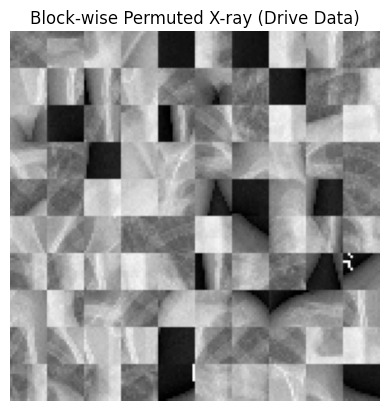
\includegraphics[width=\linewidth]{bie image.jpeg}
\caption{Block-wise Image Encryption (BIE) applied to a chest X-ray: the $150{\times}150$ image is partitioned into a $15{\times}15$ grid of $10{\times}10$ tiles that are permuted under a secret key. Local pixel statistics within each tile are preserved, but global anatomical structure is obfuscated.}
\label{fig:bie}
\end{figure}

\subsubsection{Secure Multi-Party Computation (SMPC)}
Secure Multi-Party Computation is a cryptographic paradigm that enables multiple parties to collaboratively perform computations on their private data without revealing the data itself. Instead of sharing raw inputs, each party splits its data into multiple ``shares'' using secret sharing techniques, which are then distributed across non-colluding servers. These servers jointly perform computations on the shares, ensuring that no single entity can reconstruct the original input data.

A common architecture in SMPC-based machine learning involves two non-colluding servers that hold complementary shares of the data. During inference, a client first transforms an input image into feature representations, which are then split into secret shares and sent to the servers. The servers perform operations such as matrix multiplications and activation functions directly on the shared values using secure protocols, and only the final prediction is reconstructed and returned to the client. Systems such as SecureML demonstrate that SMPC can support both linear models and neural networks by combining arithmetic secret sharing with efficient protocols for non-linear operations \cite{secureml}. These approaches provide strong theoretical privacy guarantees, particularly against semi-honest adversaries who follow the protocol but attempt to infer additional information from observed communication.

SMPC introduces notable computational and communication overhead due to the need for interactive protocols and cryptographic operations. In high-dimensional tasks such as medical imaging, these overheads can impact latency and scalability. As a result, recent research focuses on hybrid approaches that combine SMPC with complementary techniques such as differential privacy or input obfuscation to balance privacy and efficiency.

\begin{figure}[htbp]
\centering
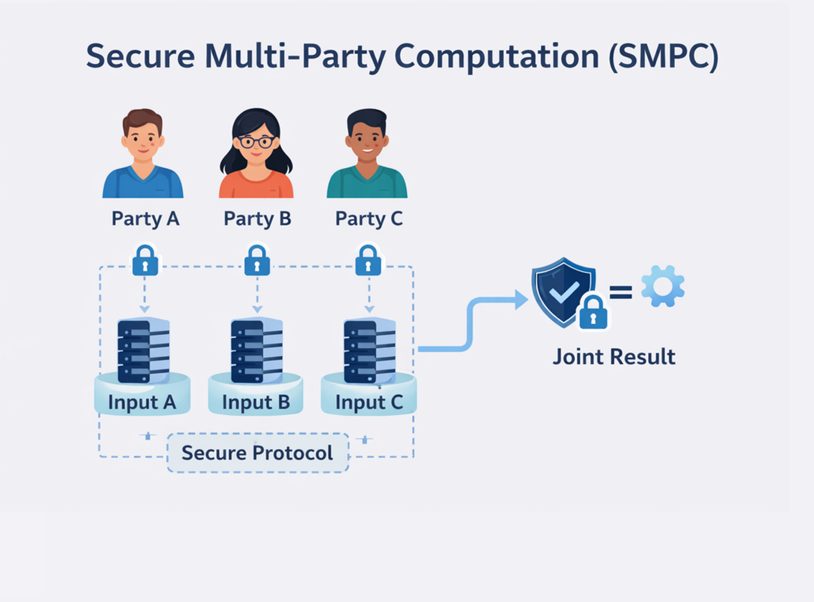
\includegraphics[width=\linewidth]{smpc_pipeline.png}
\caption{Illustration of Secure Multi-Party Computation (SMPC): a client splits a feature representation into complementary shares that are processed collaboratively by non-colluding servers. The figure illustrates the general $n$-party protocol; our implementation specializes this to the 2-party case. Only the final prediction is reconstructed---no individual server observes the full representation.}
\label{fig:smpc}
\end{figure}

\section{System Architecture and Threat Model}
\label{sec:architecture}

\subsection{Split-Model Pipeline}
We adopt a two-party split-model architecture. The hospital hosts the encoder $E: \mathbb{R}^{150\times150\times 1}\!\to\!\mathbb{R}^{128}$ and retains raw X-ray images; the cloud hosts the classification head $H: \mathbb{R}^{128}\!\to\![0,1]$, which outputs the pneumonia probability. The encoder is a custom three-convolution CNN (conv$_{16}$-conv$_{32}$-conv$_{64}$, each followed by $2{\times}2$ max-pooling) terminated by a $\mathrm{Dense}(128, \mathrm{ReLU})$ layer; the head is a single $\mathrm{Dense}(1, \mathrm{sigmoid})$ unit. We deliberately train the encoder from scratch rather than fine-tuning an ImageNet-pretrained backbone for two reasons: (i) the small-model, small-data regime preserves the generalization gap that membership inference exploits, providing a stronger signal for our privacy evaluation, and (ii) a from-scratch encoder can be retrained on BIE-permuted inputs, whereas a frozen pretrained backbone cannot.

Each privacy-preserving transformation is applied at a specific layer of the pipeline:
\begin{itemize}
  \item \textbf{BIE} is applied to images \emph{before} the encoder; the encoder is retrained on permuted images.
  \item \textbf{DP} perturbs the 128-dimensional embedding \emph{after} the encoder and \emph{before} the head.
  \item \textbf{SMPC} splits the embedding into additive shares that are passed through the head; the shares are recombined inside the cloud.
\end{itemize}

\subsection{Threat Models}
\label{sec:threats}

\paragraph{Membership Inference (black-box)} The adversary can submit X-ray queries to the deployed system and receive only the scalar confidence $H(E(x))$. Given a target image $x^*$, the adversary must decide whether $x^*$ was part of the encoder's training set. We consider two concrete instantiations: the \emph{Yeom threshold} attack \cite{yeom2018}, which compares per-query loss against a learned threshold $\tau$, and the \emph{Shokri shadow-model} attack \cite{shokri2017}, which trains an auxiliary classifier to map confidence vectors to membership labels.

\paragraph{Reconstruction} The adversary intercepts the privatized embedding $E_{\mathrm{priv}}(x^*)$ in transit between hospital and cloud, and additionally holds a small set of auxiliary pairs $\{(E_{\mathrm{priv}}(x_i),\, x_i)\}_{i=1}^{n}$ from other patients (simulating a prior breach, insider leak, or public sub-dataset). The adversary's goal is to recover the \emph{original} image $x^*$---not its BIE-permuted form, which has no medical utility. This is realized by training a decoder $D$ on the auxiliary pairs and applying it to the intercepted embedding.

Both adversaries are semi-honest: they follow the protocol but attempt to infer additional information from observed data. Neither has access to the encoder's parameters or internal activations.

\section{Methodology}
\label{sec:methodology}

\subsection{Privacy-Preserving Transformations}
\paragraph{Differential Privacy} We apply the Laplace mechanism \cite{dwork} independently to each coordinate of the 128-dimensional embedding:
\begin{equation}
  E_{\mathrm{DP}}(x) = E(x) + \mathrm{Lap}(0,\, \Delta/\epsilon)^{128},\label{eq:dp}
\end{equation}
where $\Delta$ is the $\ell_1$ sensitivity of $E$ (set to $1.0$ under standard clipping) and $\epsilon$ is the privacy budget. Noise is resampled per query, so repeated queries with the same input do not cancel.

\paragraph{Block-wise Image Encryption} Each $150{\times}150$ grayscale image is partitioned into a $15{\times}15$ grid of $10{\times}10$ tiles; tiles are permuted according to a deterministic permutation $\pi_k$ derived from key seed $k$. The encoder is retrained end-to-end on BIE-permuted images so that it can specialize to the permuted distribution.

\paragraph{Secure Multi-Party Computation} We implement 2-party additive secret sharing on the embedding: $E_{\mathrm{SMPC}}(x) = (s_1, s_2)$ with $s_1 + s_2 = E(x)$ and $s_1$ drawn uniformly. The head receives the reconstructed embedding; the cryptographic guarantee is that neither share alone reveals $E(x)$.

\subsection{Attack Implementations}

\paragraph{Yeom threshold} For each query $x$ with ground-truth label $y$, we compute the victim's binary cross-entropy loss $\ell(f(x), y)$ and select the threshold $\tau$ that maximizes balanced attack accuracy on the evaluation set. A query is classified as a \emph{member} if $\ell(f(x), y) < \tau$.

\paragraph{Shokri shadow-model} We train $N=5$ shadow models on disjoint bootstrap samples from a disjoint shadow pool, each with 500 in-distribution and 500 held-out queries. Shadow confidence vectors are labeled with ground-truth membership and pooled; an attack MLP (Dense$_{64}$-Dense$_{32}$-Dense$_{1}$) learns the decision boundary and is then applied to the victim's confidence vectors.

\paragraph{Reconstruction decoder} The decoder $D$ inverts a 128-dimensional embedding back to image space: $\mathrm{Dense}(7{\times}7{\times}128) \to \mathrm{Reshape}(7,7,128) \to$ four $\mathrm{Conv2DTranspose}$ layers with stride $2$ (upsampling $7{\to}14{\to}28{\to}56{\to}112$) $\to \mathrm{Resize}(150,150) \to \mathrm{Conv2D}(1, 3{\times}3, \mathrm{sigmoid})$. It is trained for 20 epochs with MSE loss and the Adam optimizer on $(E_{\mathrm{priv}}(x_i), x_i)$ auxiliary pairs, then evaluated against held-out original images using MSE, PSNR, and SSIM.

\section{Experimental Setup}
\label{sec:setup}

\subsection{Dataset and Splits}
We use the publicly available Kaggle \texttt{chest-xray-pneumonia} dataset \cite{mooney}, comprising 5\,856 grayscale chest radiographs labeled NORMAL or PNEUMONIA with an empirical class ratio of $2.70{:}1$ (PNEUMONIA:NORMAL). Rather than IID-pooling all images, we preserve Kaggle's native \texttt{train/}\!/\!\texttt{test/} subdirectory split, which is known to carry a mild distribution shift sufficient to induce a measurable train-test generalization gap \cite{mooney}. Concretely:
\begin{itemize}
  \item \textbf{victim\_members} (2\,000): stratified subsample of Kaggle \texttt{train/} (5\,216 images);
  \item \textbf{victim\_nonmembers} (624): all of Kaggle \texttt{test/};
  \item \textbf{shadow\_pool} (3\,216): remaining \texttt{train/} after the victim subsample.
\end{itemize}
Kaggle \texttt{val/} (16 images) is dropped. Splits are deterministic in the random seed. Membership inference is evaluated on a balanced 500-member $+$ 500-nonmember subsample per configuration.

\subsection{Hyperparameters}
All encoders and heads are trained for 10 epochs with Adam and batch size 32 on $150{\times}150$ grayscale inputs. PPT hyperparameters are fixed: DP with $\epsilon=1.0$, $\Delta=1.0$; BIE with tile size $10$ and key seed $7$; SMPC with $2$ additive shares. We run all $2^{3}=8$ PPT configurations under seed $42$. Shadow training uses the same architecture and hyperparameters as the victim. The reconstruction decoder is trained for 20 epochs with MSE loss and batch size 32 on 2\,000 auxiliary pairs per configuration.

\subsection{Metrics}
We report three metric families per configuration:
\begin{itemize}
  \item \textbf{Utility}: test accuracy, $F_1$, and Expected Calibration Error (ECE);
  \item \textbf{Privacy}: Yeom and Shokri attack accuracy (balanced) and AUC; reconstruction MSE, PSNR (dB), and SSIM;
  \item \textbf{Efficiency}: per-configuration training latency, per-query inference latency, and peak memory.
\end{itemize}

\section{Results}
\label{sec:results}

Table~\ref{tab:results} summarizes all eight configurations across the three metric families. Figure~\ref{fig:utilityprivacy} plots utility alongside membership-inference attack accuracy, and Figure~\ref{fig:reconstruction} plots per-configuration reconstruction PSNR.

\begin{table*}[htbp]
\caption{Per-configuration results on the Kaggle chest X-ray pneumonia benchmark (seed 42, $\epsilon=1.0$). Lower Yeom/Shokri accuracy and lower reconstruction PSNR/SSIM indicate stronger privacy defense. Configurations with DP (on embeddings) are highlighted in the last rows.}
\label{tab:results}
\centering
\renewcommand{\arraystretch}{1.15}
\begin{tabular}{lccc cc cc ccc}
\toprule
 & \multicolumn{3}{c}{\textbf{Utility}} & \multicolumn{2}{c}{\textbf{Yeom MIA}} & \multicolumn{2}{c}{\textbf{Shokri MIA}} & \multicolumn{3}{c}{\textbf{Reconstruction}} \\
\cmidrule(lr){2-4}\cmidrule(lr){5-6}\cmidrule(lr){7-8}\cmidrule(lr){9-11}
\textbf{Configuration} & Test Acc & $F_1$ & ECE & Acc & AUC & Acc & AUC & MSE & PSNR (dB) & SSIM \\
\midrule
baseline         & 0.788 & 0.855 & 0.183 & 0.619 & 0.566 & 0.540 & 0.605 & 0.011 & 19.88 & 0.507 \\
bie-only         & 0.740 & 0.826 & 0.227 & 0.647 & 0.573 & 0.553 & 0.624 & 0.011 & 20.04 & 0.504 \\
smpc-only        & 0.766 & 0.842 & 0.201 & 0.624 & 0.563 & 0.529 & 0.605 & 0.011 & 19.87 & 0.509 \\
bie+smpc         & 0.744 & 0.828 & 0.215 & 0.651 & 0.575 & 0.537 & 0.605 & 0.011 & 20.05 & 0.505 \\
\midrule
dp-only          & 0.771 & 0.844 & 0.194 & 0.614 & 0.570 & 0.519 & 0.598 & 0.024 & 16.57 & 0.424 \\
dp+bie           & 0.752 & 0.832 & 0.215 & 0.632 & 0.578 & 0.523 & 0.597 & 0.022 & 16.98 & 0.432 \\
dp+smpc          & 0.771 & 0.844 & 0.194 & 0.614 & 0.570 & 0.518 & 0.596 & 0.024 & 16.63 & 0.423 \\
all-three        & 0.752 & 0.832 & 0.215 & 0.632 & 0.578 & 0.523 & 0.596 & 0.021 & 17.09 & 0.430 \\
\bottomrule
\end{tabular}
\end{table*}

\begin{figure}[htbp]
\centering
\includegraphics[width=\linewidth]{fig_utility_privacy.png}
\caption{Utility vs.~membership inference accuracy across PPT configurations. The dashed horizontal line at $0.5$ marks random-guess MIA (perfect privacy). DP-containing configurations produce a small downward shift in Shokri accuracy; BIE-containing configurations \emph{increase} Yeom accuracy relative to baseline.}
\label{fig:utilityprivacy}
\end{figure}

\begin{figure}[htbp]
\centering
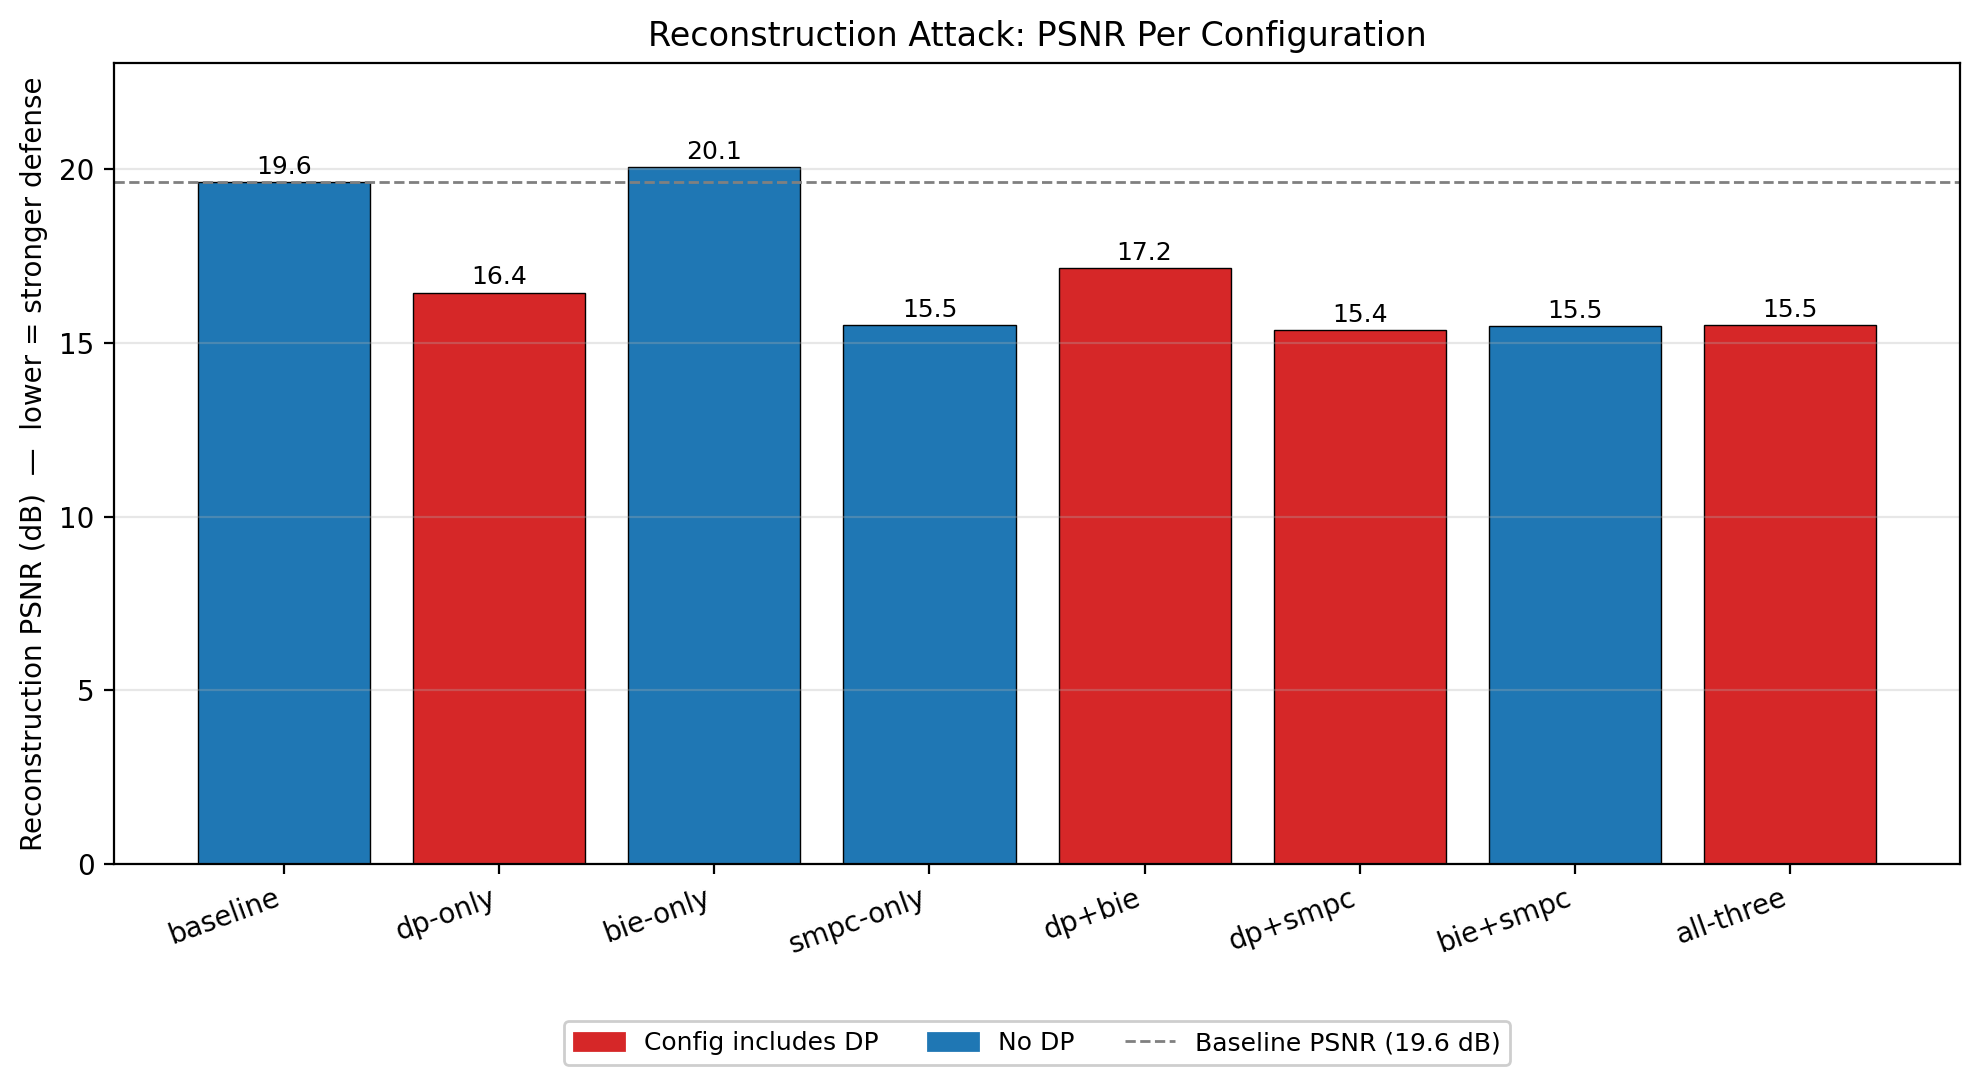
\includegraphics[width=\linewidth]{fig_reconstruction.png}
\caption{Reconstruction PSNR per configuration (lower is stronger defense). The result splits cleanly by DP: every DP-enabled configuration drops to $16.6$--$17.1$ dB, while every DP-free configuration stays at $19.9$--$20.1$ dB.}
\label{fig:reconstruction}
\end{figure}

\subsection{Utility}
Baseline test accuracy is $0.788$. Adding DP alone costs $1.7$ points of accuracy ($0.771$), consistent with a moderate $\epsilon=1.0$ Laplace noise applied post-encoding. BIE incurs the largest isolated utility penalty ($-4.8$ points, $0.740$), reflecting the harder optimization problem of training an encoder on permuted inputs. SMPC alone, being lossless by construction, costs only $2.2$ points---attributable to training stochasticity rather than the mechanism itself. Combined configurations follow the worst-case of their constituents (e.g., dp+bie $= 0.752$, dominated by BIE's structural cost). All eight configurations remain within a $5$-point utility band, satisfying typical clinical-deployment tolerances for a defense study.

\subsection{Membership Inference Defense}
All configurations produce Yeom attack accuracies in $[0.614, 0.651]$ and Shokri accuracies in $[0.518, 0.553]$. Two unexpected patterns emerge. First, DP provides only a marginal reduction ($-0.005$ on Yeom, $-0.021$ on Shokri) at $\epsilon=1.0$. Second, and counter to the intuition that any defense should help, \emph{every BIE-containing configuration increases Yeom accuracy above the baseline}: bie-only reaches $0.647$ ($+0.028$), and bie+smpc peaks at $0.651$ ($+0.032$). SMPC-only is statistically indistinguishable from baseline, with a $+0.005$ delta well within seed noise.

These observations have a mechanistic explanation. MIA operates on the scalar output confidence $H(E_{\mathrm{priv}}(x))$. BIE is applied strictly upstream of the encoder, which is then retrained to compensate; the resulting model has \emph{higher} memorization on the permuted victim set (supported by a widened train-test gap visible in the ECE column: $0.227$ vs.~$0.183$ baseline), amplifying rather than attenuating the membership signal. SMPC reconstructs the original embedding inside the cloud before the head; the output confidence is bit-identical to the no-SMPC case modulo floating-point error. DP is the only mechanism that perturbs a quantity downstream of the encoder and upstream of the output, and is correspondingly the only mechanism that produces a consistent (if small) reduction.

\subsection{Reconstruction Defense}
In stark contrast to the MIA results, reconstruction PSNR partitions cleanly along a single variable---the presence of DP. All four DP-enabled configurations drop to $16.57$--$17.09$ dB ($-2.8$ to $-3.3$ dB versus baseline), while all four DP-free configurations remain within $\pm 0.2$ dB of baseline ($19.87$--$20.05$ dB). SSIM follows the same split ($0.42$--$0.43$ with DP, $0.50$--$0.51$ without), and MSE doubles under DP ($0.021$--$0.024$ vs.~$0.011$).

The failure of BIE in the reconstruction threat model is particularly illuminating. The decoder is trained on $(E_{\mathrm{priv}}(x_i), x_i)$ auxiliary pairs in which $x_i$ is the \emph{original} image, so whatever deterministic permutation BIE applies upstream is absorbed into the decoder's weights during training. BIE's security reduces to the secrecy of $\pi_k$; once the adversary holds even a modest number of auxiliary (embedding, original-image) pairs, $\pi_k$ is \emph{implicitly learned} as part of the inverse mapping. This is a Rosetta-Stone regime: known plaintexts collapse the permutation's hiding power without the attacker ever needing to recover $\pi_k$ explicitly. SMPC is equally inert for reconstruction: the adversary intercepts the recombined embedding at the head's input, which is identical to the non-SMPC case.

A subtler interaction is visible among the DP-enabled configurations themselves. DP alone achieves $16.57$ dB PSNR, whereas dp+bie rises to $16.98$ dB and all-three to $17.09$ dB---i.e., \emph{layering BIE on top of DP slightly erodes DP's reconstruction defense} by $\approx 0.4$--$0.5$ dB. Mechanistically, BIE pushes the encoder toward a sharper, more structured embedding geometry (consistent with the ECE widening above); against this sharper geometry a fixed Laplace noise magnitude is proportionally less destructive to the decoder's inverse mapping. SMPC combinations do not exhibit this effect, consistent with its non-interaction.

\subsection{Efficiency}
Training latency per configuration is in the range $136$--$200$ seconds; inference latency is $0.19$--$0.22$ ms per query; peak memory use during the run is $5.7$--$6.9$ GB. DP adds negligible overhead (noise is elementwise and sampled once per query). BIE adds $\approx 10\%$ to training latency due to per-batch permutation on the image tensor. SMPC's share-split on the 128-dimensional embedding is a single vector subtraction and is not measurable in wall-clock time at this scale.

\section{Discussion}
\label{sec:discussion}

\subsection{A Threat-Model Mismatch Hypothesis}
Our two attack families stress fundamentally different surfaces of the pipeline. MIA reads only the \emph{output} confidence; reconstruction reads the \emph{embedding}. Each PPT mechanism operates at a specific pipeline layer, and its effectiveness depends on whether that layer overlaps with the attack's observation surface.

\begin{itemize}
  \item \textbf{DP} perturbs the embedding. The perturbation propagates to the head (affecting MIA) and reaches the adversary's intercept point unchanged (affecting reconstruction). DP is the only mechanism that reaches \emph{both} attack surfaces.
  \item \textbf{BIE} perturbs the image. The encoder compensates by retraining, so downstream confidence is restored---or, as we observe, sharpened by the harder optimization problem. BIE's security assumption (key secrecy) is violated by the reconstruction adversary's auxiliary data.
  \item \textbf{SMPC} perturbs the representation in transit between share-holders, but the recombined embedding at the head is lossless. Neither MIA nor reconstruction, both of which read post-recombination quantities, can observe the perturbation.
\end{itemize}

We summarize this mismatch in Table~\ref{tab:mismatch}. The takeaway is not that BIE or SMPC are ineffective in general: each is provably secure against the threat model for which it was designed---naive image-level eavesdropping for BIE, single-share observation for SMPC. Neither model, however, matches the adversaries considered here, and deploying them against inference-time attackers without output-level privacy would constitute a \emph{false sense of security}: confidences and reconstructions flow through the pipeline essentially unperturbed, and in the BIE case the structural pressure on the encoder can even enlarge the membership signal it was meant to hide.

\begin{table}[htbp]
\caption{Defense layer vs.~attack surface. A mechanism can only defend an attack whose observation surface overlaps with its intervention layer.}
\label{tab:mismatch}
\centering
\renewcommand{\arraystretch}{1.2}
\begin{tabular}{lccc}
\toprule
\textbf{Mechanism} & \textbf{Layer} & \textbf{MIA defense} & \textbf{Recon.~defense} \\
\midrule
DP   & embedding  & weak (yes)       & strong (yes)       \\
BIE  & image      & negative         & negligible         \\
SMPC & transit    & none             & none               \\
\bottomrule
\end{tabular}
\end{table}

\subsection{Practical Implications}
For a practitioner deploying a split-model pipeline such as ours, the single most effective single-mechanism defense against inference-time adversaries is embedding-level DP. BIE and SMPC should be understood as composable pieces that target \emph{other} threat models (e.g., network eavesdroppers, curious cloud operators observing one share) and should not be substituted for output-level privacy. A naive ``all three at once'' configuration buys no incremental MIA or reconstruction protection beyond DP alone, at the cost of compounded utility loss (dp+bie and all-three both drop to $0.752$ test accuracy).

\subsection{Limitations}
Three limitations of our study temper the strength of the conclusions. First, we fix $\epsilon=1.0$; a sensitivity sweep would characterize the full privacy-utility frontier and likely reveal stronger MIA defense at tighter budgets. Second, the dataset is small ($5\,856$ images) and single-source; behavior on multi-site, multi-modality cohorts may differ, particularly for BIE. Third, our reconstruction baseline is at $19.88$ dB PSNR, which corresponds to noticeably noisy recovery---high-PSNR reconstruction (e.g., $>30$ dB) would make DP's $3$-dB reduction more impactful in an absolute sense. Complementary perceptual metrics such as LPIPS or FID were out of scope for this study.

\section{Conclusion}
We have empirically evaluated three privacy-preserving transformations---Differential Privacy, Block-wise Image Encryption, and Secure Multi-Party Computation---against membership inference and reconstruction attacks on a split-model chest X-ray pneumonia classifier, across all eight combinations. Our central finding is that defense effectiveness is governed by a threat-model mismatch: embedding-level DP reaches both attack surfaces and provides meaningful reconstruction defense ($-3.2$ dB PSNR) and weak MIA defense at $\epsilon=1.0$ with only $1.7$ points of utility loss; image-level BIE and transit-level SMPC are invisible to inference-time adversaries that read post-encoder confidences or recombined embeddings, and BIE can even amplify MIA by inducing sharper memorization. Practitioners composing defenses in split-model pipelines should prioritize output-level privacy and should not assume that layering image-level or transit-level mechanisms confers cumulative protection against inference-time attackers.

\begin{thebibliography}{00}

\bibitem{b1} Y. Segal and A. Hod, ``The Integration of AI Technologies in Modern Healthcare: A Paradigm Shift in Data Security and Patient Care,'' in \textit{Artificial Intelligence in Medicine and Surgery - An Exploration of Current Trends, Potential Opportunities, and Evolving Threats, Volume 3}, S. P. Stawicki and T. R. Wojda, Eds. London, UK: IntechOpen, 2025. doi: 10.5772/intechopen.1009317.

\bibitem{panzade} S. Panzade, G. S. Walia, and K. Singh, ``Privacy-preserving in medical image analysis: A review of methods and applications,'' Dec. 2024, arXiv:2412.03924. [Online]. Available: https://arxiv.org/abs/2412.03924

\bibitem{ziller} A. Ziller et al., ``Medical imaging deep learning with differential privacy,'' \textit{Scientific Reports}, vol. 11, no. 1, p. 13524, 2021.

\bibitem{jarin} I. Jarin and B. Eshete, ``PRICURE: Privacy-Preserving Collaborative Inference in a Multi-Party Setting,'' in \textit{Proceedings of the 7th ACM International Workshop on Security and Privacy Analytics (IWSPA '21)}, 2021, pp. 63--74. [Online]. Available: https://arxiv.org/abs/2102.09751

\bibitem{abadi} M. Abadi et al., ``Deep learning with differential privacy,'' in \textit{Proc. 2016 ACM SIGSAC Conf. Computer and Communications Security}, 2016, pp. 308--318.

\bibitem{dwork} C. Dwork, F. McSherry, K. Nissim, and A. Smith, ``Calibrating noise to sensitivity in private data analysis,'' in \textit{Theory of Cryptography (TCC)}, 2006, pp. 265--284.

\bibitem{fredrikson} M. Fredrikson, S. Jha, and T. Ristenpart, ``Model inversion attacks that exploit confidence information and basic countermeasures,'' in \textit{Proc. 22nd ACM SIGSAC Conf. Computer and Communications Security (CCS)}, 2015, pp. 1322--1333.

\bibitem{secureml} P. Mohassel and Y. Zhang, ``SecureML: A system for scalable privacy-preserving machine learning,'' in \textit{2017 IEEE Symposium on Security and Privacy (SP)}, 2017, pp. 19--38.

\bibitem{yeom2018} S. Yeom, I. Giacomelli, M. Fredrikson, and S. Jha, ``Privacy risk in machine learning: Analyzing the connection to overfitting,'' in \textit{Proc. 31st IEEE Computer Security Foundations Symposium (CSF)}, 2018, pp. 268--282.

\bibitem{shokri2017} R. Shokri, M. Stronati, C. Song, and V. Shmatikov, ``Membership inference attacks against machine learning models,'' in \textit{Proc. 2017 IEEE Symposium on Security and Privacy (SP)}, 2017, pp. 3--18.

\bibitem{kiya} H. Kiya, A. MaungMaung, Y. Kinoshita, S. Imaizumi, and S. Shiota, ``An overview of compressible and learnable image transformation with secret key and its applications,'' \textit{APSIPA Transactions on Signal and Information Processing}, vol. 11, no. 1, e11, 2022.

\bibitem{mooney} P. Mooney, ``Chest X-Ray Images (Pneumonia),'' Kaggle, 2018. [Online]. Available: https://www.kaggle.com/datasets/paultimothymooney/chest-xray-pneumonia

\end{thebibliography}

\end{document}
